\section{Use case 5: Traffic flow modeling}
\label{sec:traffic-flow}

\paragraph{Problem statement}
Macroscopic traffic models describe the evolution of vehicle density
$\rho(x,t)$ along a road. In the Lighthill--Whitham--Richards (LWR) model,
density satisfies the scalar conservation law
\begin{equation}
    \partial_t \rho + \partial_x q(\rho) = 0,
    \label{eq:traffic-lwr}
\end{equation}
where the fundamental diagram $q(\rho)$ relates density to traffic flux and
the corresponding velocity is $v(\rho)=q(\rho)/\rho$. Classical fundamental
diagrams provide compact and physically interpretable constitutive laws, but a
fixed analytical form can retain systematic bias when it is embedded in a
spatio-temporal traffic simulation. Replacing the diagram entirely with a
flexible data-driven model may improve fit at the cost of interpretability and
physical structure.

We therefore considered the intermediate hypothesis that a calibrated
classical diagram captures the principal traffic physics, while its remaining
bias can be represented by a compact multiplicative correction,
\begin{equation}
    q_{\mathrm{corr}}(\rho)
    = q_{\mathrm{base}}(\rho;\boldsymbol{\theta})
      g(\rho;\boldsymbol{c}).
    \label{eq:traffic-correction}
\end{equation}
Here $q_{\mathrm{base}}$ is one of five established diagrams---Greenshields,
the equilibrium Intelligent Driver Model (IDM), Weidmann, Triangular, or Del
Castillo---whose calibrated coefficients $\boldsymbol{\theta}$ remain fixed
during structural discovery. The correction $g$ is dimensionless, and
$g=1$ recovers the unmodified diagram. Restricting the selected corrections to
positive exponential multipliers preserves the units, sign, and zeros of the
baseline flux, while still allowing local and short-range spatial adjustments.

\paragraph{Method}
The \texttt{automodel} skill was used with OpenAI Codex with the following
domain-specific choices on top of the baseline workflow. The implementation,
configurations, and reproducibility materials are available in the
\href{https://github.com/cpml-au/automodel-traffic}{\texttt{automodel-traffic}
repository}.

\noindent\textbf{(i) Objective and data splitting.}
We used density, velocity, and flow measurements from the NGSIM Interstate~80
data set. After nondimensionalization, the data comprise 79 spatial rows and
180 time samples; 75 interior spatial positions enter the objective. The split
was chronological and fixed before model discovery: samples 0--63 were used to
fit correction coefficients, samples 64--107 for structural validation and
model selection, and samples 108--179 as a final held-out test interval. No
shuffling was used. The two component errors are relative $L_2$ errors,
\begin{equation}
    E_\rho = \frac{\lVert\widehat{\rho}-\rho\rVert_2}
                        {\lVert\rho\rVert_2},
    \qquad
    E_v = \frac{\lVert\widehat{v}-v\rVert_2}
                    {\lVert v\rVert_2},
\end{equation}
and candidate fit was summarized by
\begin{equation}
    E_{\mathrm{data}} = 50\left(E_\rho^2+E_v^2\right).
    \label{eq:traffic-data-error}
\end{equation}
Structure selection used validation
$E_{\mathrm{fitness}}=E_{\mathrm{data}}+0.01n$, where $n$ is the number of
nodes in the expression tree. Thus, an added mechanism had to offset its
complexity cost rather than merely produce a numerically negligible reduction
in residual error.

\noindent\textbf{(ii) Model and evaluator.}
A candidate model was a multiplier $g$ applied to one of the five fixed
fundamental diagrams in Eq.~\eqref{eq:traffic-correction}. Each candidate was
evaluated by solving Eq.~\eqref{eq:traffic-lwr} with the same initial state,
measured boundary density, mesh, and time refinement as its baseline. The
finite-volume update used a Rusanov/Godunov flux implemented with discrete
exterior calculus operators. For nonlocal corrections, the wave-speed bound
included the off-diagonal terms of the flux Jacobian, rather than treating a
spatially coupled flux as pointwise.

The coefficient optimizer used deterministic bounded Powell searches with
explicit starts and evaluation budgets. Candidates were rejected if their
multipliers or simulations were non-finite, if they produced a non-positive
multiplier or negative velocity on the relevant physical density domain, or if
the corrected velocity violated the prescribed monotonicity check. Every
expression, parameter vector, train/validation score, feasibility result,
runtime, and memory measurement was retained.

\noindent\textbf{(iii) Structural search and confirmation.}
The search used $M\times S\times I=5\times3\times3$: five meta-iterations,
three parallel hypothesis streams per iteration, and three sequential
structural attempts per stream. Every proposed structure was fitted separately
to all five baseline diagrams, giving 225 baseline--candidate fits before final
refitting. Early iterations explored positive pointwise polynomial, anchored,
saturating, and rational corrections. Later iterations introduced short-range
convolutions and Hodge-star features defined on the traffic mesh, and refined
the most promising incumbents. Shortlisted candidates were re-evaluated in the
root process before acceptance, and the test interval was not accessed during
this search.

Let
\begin{equation}
    S_3(\rho)=\operatorname{conv}_3(\rho,\mathbf{1}),
    \qquad
    C(\rho)=S_3(\rho)-3\operatorname{conv}_1(\rho,\mathbf{1}),
\end{equation}
where $C$ is a local density-contrast feature, and let $H_2(\rho)$ denote the
quadratic Hodge-star feature obtained by squaring the dual one-cochain
$\star\rho$ and mapping it back to primal nodes. Validation selected the
following baseline-specific structures:
\begin{align}
    g_{\mathrm{G}}(\rho)
        &= \exp\!\left(c_0+a\rho+b\rho^2+dC(\rho)\right), \\
    g_{\mathrm{IDM}}(\rho)
        &= \exp\!\left(aC(\rho)+bH_2(\rho)C(\rho)\right), \\
    g_{\mathrm{W}}(\rho)
        &= \exp\!\left(a\rho\left(1-\rho/\rho_{\max}\right)\right), \\
    g_{\mathrm{T}}(\rho)
        &= \exp\!\left(a\rho C(\rho)\right), \\
    g_{\mathrm{DC}}(\rho)
        &= \exp\!\left(c_0+aS_3(\rho)+bC(\rho)\right).
    \label{eq:traffic-selected-corrections}
\end{align}
These structures admit a direct physical reading. Because every $g$ is a
positive multiplier, a correction changes the magnitude of the baseline flux
and velocity without changing the baseline's zero-flow states. The contrast
$C$ vanishes in a spatially homogeneous state, so terms containing $C$ act
only where the density varies over the short convolution window. They can
therefore be interpreted as compact non-equilibrium corrections at developing
traffic fronts, rather than as changes to the homogeneous fundamental diagram.

The refitted Greenshields coefficients have $c_0>0$ and $a,b,d<0$. The
constant term raises the low-density branch, the negative linear and quadratic
terms progressively temper this uplift as density increases, and the contrast
term adjusts the flux near spatial transitions. This supplements the rigid
parabolic Greenshields curve with both density-dependent curvature and a local
traffic-state correction. For IDM, both fitted coefficients are negative and
the correction is proportional to $C$; the non-negative Hodge feature $H_2$
modulates the strength of that response with local traffic loading. The model
therefore leaves uniform flow unchanged but reacts more strongly to density
variations in heavily loaded states, consistent with a queue-front or
anticipation effect absent from an equilibrium closure.

The Weidmann correction is the most directly interpretable. Its fitted
$a>0$, so it increases flux at intermediate densities while remaining exactly
one at both $
ho=0$ and $
ho=\rho_{\max}$. It preserves the free-flow and jam
limits and modifies only the interior of the diagram. The Triangular model has
$a<0$ and gates the contrast by density: it is inactive in empty or homogeneous
traffic but becomes more influential as congestion develops. Finally, the Del
Castillo fit has $c_0>0$ and $a,b<0$. It combines a small global uplift with
suppression as the three-cell density aggregate $S_3$ grows and an additional
response at spatial density contrasts. Taken together, the selected structures
suggest that the residual bias is baseline dependent: some diagrams mainly
need a correction to their homogeneous density dependence, whereas others
benefit from sensitivity to short-range traffic heterogeneity. These
interpretations are structural hypotheses, not identified driver-behaviour
mechanisms, and require validation on other roads and traffic regimes.

After these structures were frozen, their coefficients were refitted on the
combined train and validation interval (samples 0--107). Each frozen model was
then evaluated once on samples 108--179. The held-out result could not affect
either the selected structure or its coefficients.

Models were ranked by held-out $E_{\mathrm{data}}$. Improvement relative to a
model's own classical baseline was defined as
$100(E_{\mathrm{data}}^{\mathrm{base}}-E_{\mathrm{data}}^{\mathrm{model}})
/E_{\mathrm{data}}^{\mathrm{base}}$.

\paragraph{Results}
Table~\ref{tab:traffic-test-results} compares the five classical diagrams with
the corresponding structures found in the Automodel search. Automodel--Del
Castillo attained the lowest held-out density, velocity, and aggregate errors,
with $E_{\mathrm{data}}=6.780$. The Automodel--Greenshields correction produced
the largest improvement over its baseline, reducing test $E_{\mathrm{data}}$
by 23.17\%. Automodel improved held-out $E_{\mathrm{data}}$ for four of the five
baseline families; the exception was IDM, for which the score increased by
2.30\%. Figure~\ref{fig:traffic-fields} shows the measured spatio-temporal
fields beside the five Automodel predictions. The models reproduce the broad
traffic regimes but smooth part of the fine-scale variability in the data.
Figure~\ref{fig:traffic-velocity-predictions} makes the remaining velocity
error explicit: the predictions follow the central trend while compressing the
observed velocity range, particularly at its upper end.

\begin{figure}[t]
    \centering
    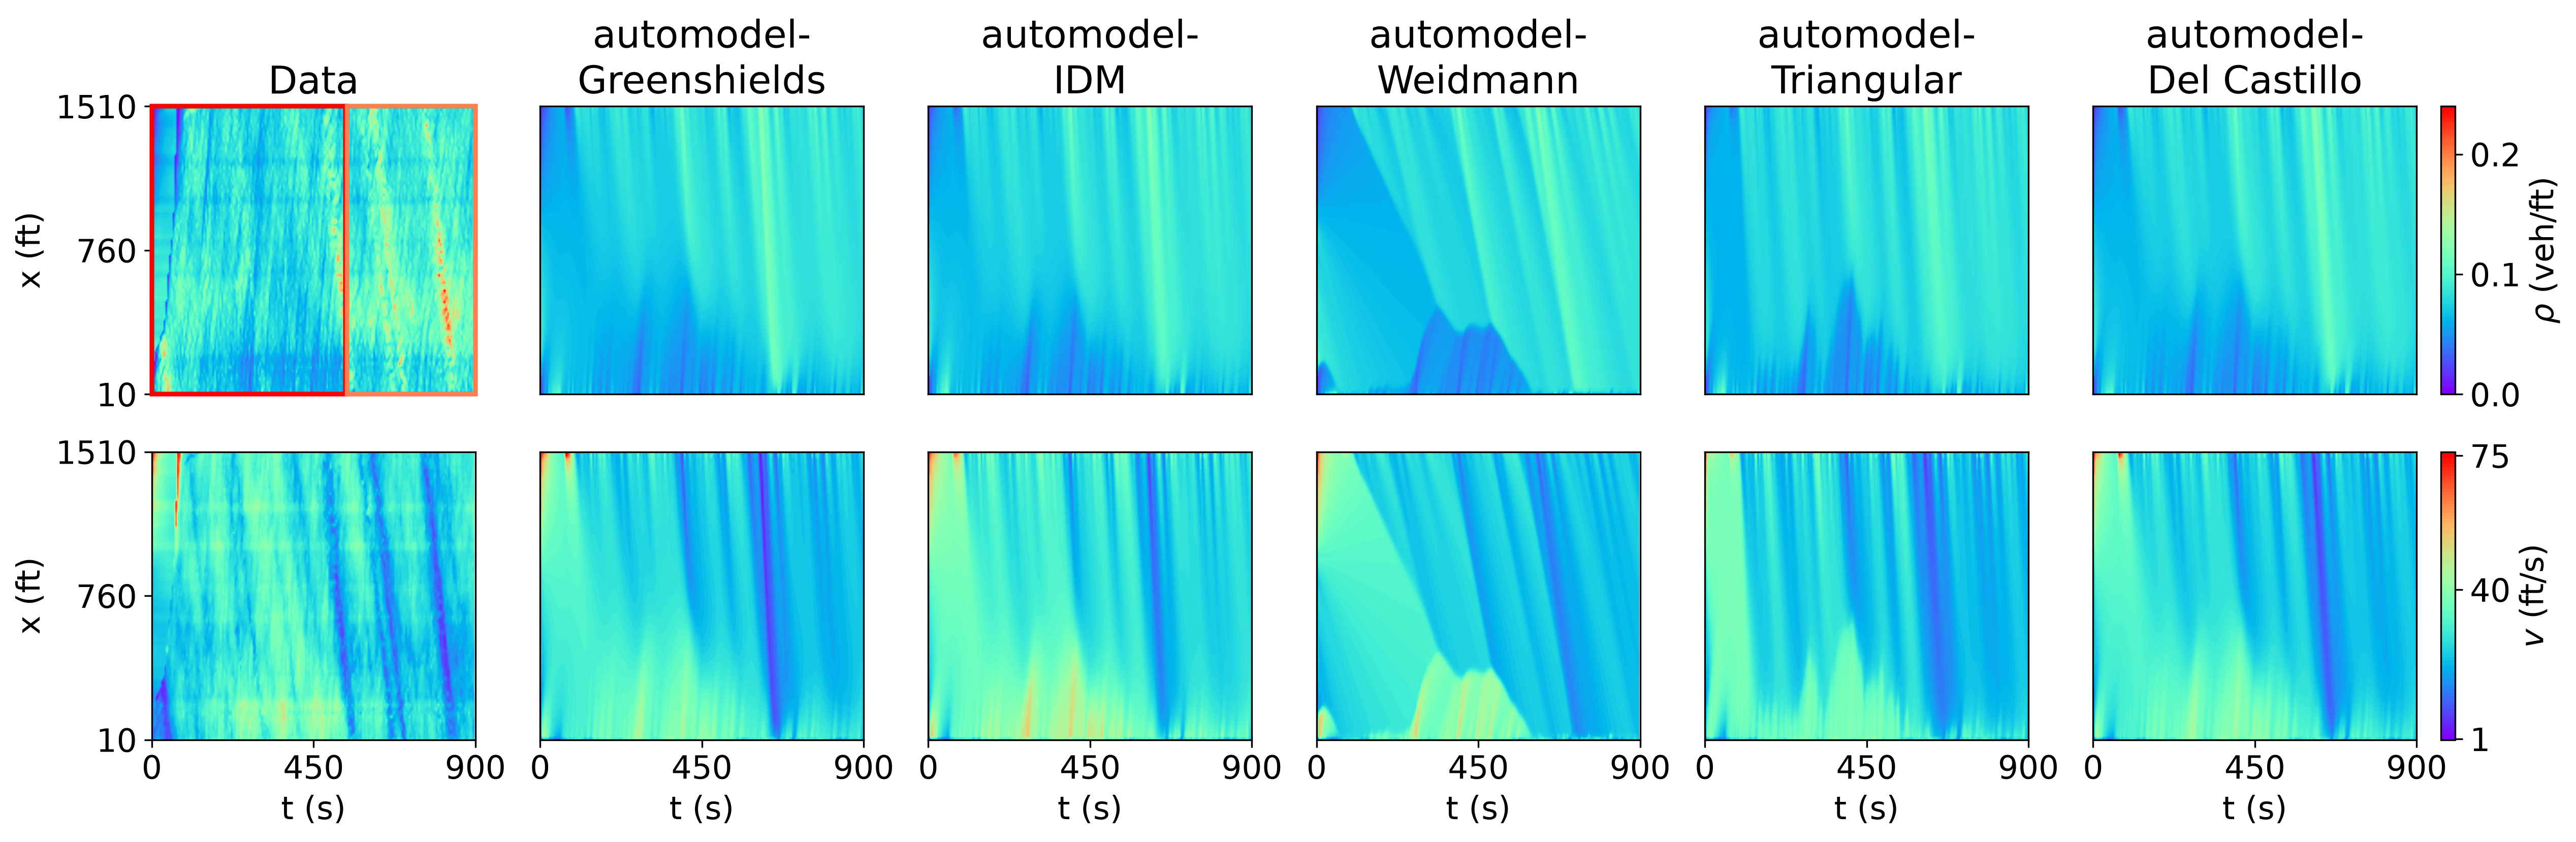
\includegraphics[width=\textwidth]
        {paper/figures/rho_v_f_plot_I80_prediction_automodel.png}
    \caption{Measured I80 fields and predictions from the five selected
    Automodel corrections. Density is shown in the top row and velocity in the
    bottom row; the first column contains the measurements and the remaining
    columns the model predictions. The outlined regions in the measured
    density panel distinguish the development and held-out time intervals.}
    \label{fig:traffic-fields}
\end{figure}

\begin{figure}[t]
    \centering
    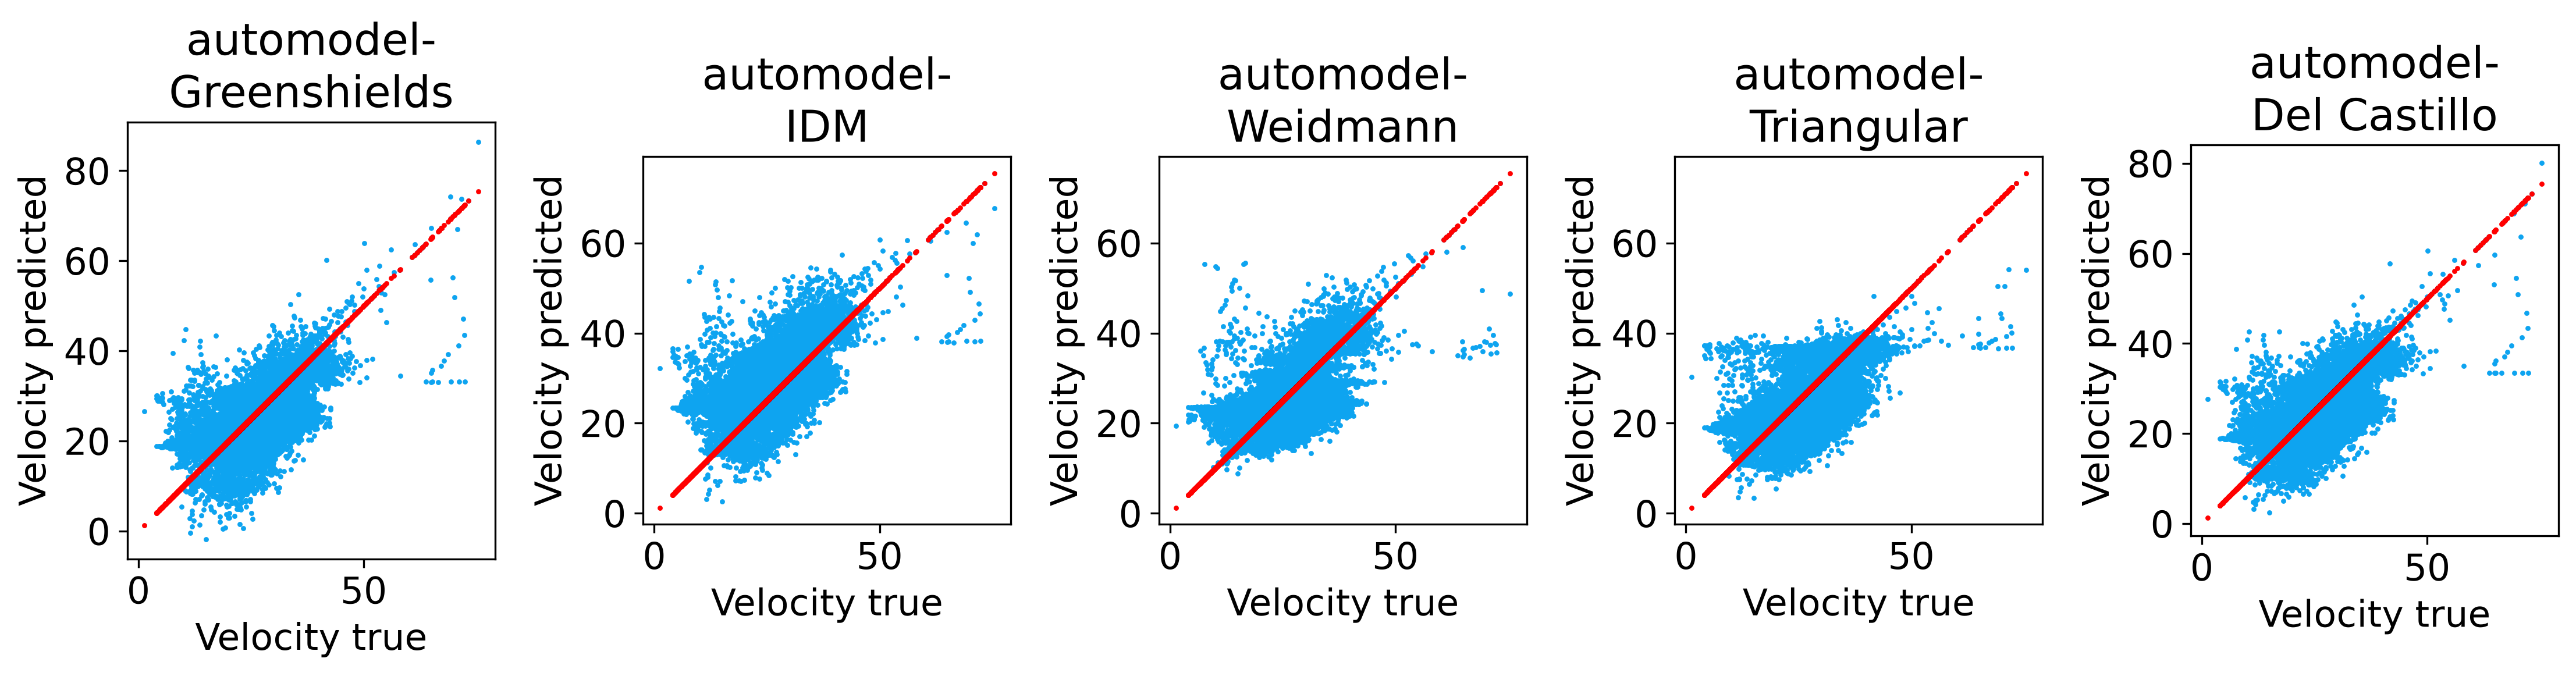
\includegraphics[width=\textwidth]
        {paper/figures/pred_actual_velocity_I80_prediction_automodel.png}
    \caption{Predicted versus measured velocity for the five selected
    Automodel corrections over the complete I80 simulation. The red diagonal
    is the identity line; departures from it show the magnitude and direction
    of the velocity residuals.}
    \label{fig:traffic-velocity-predictions}
\end{figure}

\begin{table}[t]
    \centering
    \small
    \setlength{\tabcolsep}{3.5pt}
    \caption{Held-out I80 prediction errors. Lower is better for all error
    columns. Parentheses give rank by full-precision test
    $E_{\mathrm{data}}$ across the ten models. $\Delta_{\mathrm{base}}$ is the
    percentage reduction in test $E_{\mathrm{data}}$ relative to the model's
    own classical baseline; positive values indicate improvement. AM denotes
    \texttt{automodel}.}
    \label{tab:traffic-test-results}
    \begin{tabular}{@{}lrrrr@{}}
        \toprule
        Model & $E_\rho$ & $E_v$ & $E_{\mathrm{data}}$ (rank)
              & $\Delta_{\mathrm{base}}$ \\
        \midrule
        Greenshields       & 0.294 & 0.313 & 9.230 (10) & --         \\
        AM--Greenshields   & 0.255 & 0.277 & 7.092 (3)  & $+23.17\%$ \\
        IDM                & 0.258 & 0.270 & 6.957 (2)  & --         \\
        AM--IDM            & 0.256 & 0.277 & 7.117 (4)  & $-2.30\%$  \\
        Weidmann           & 0.265 & 0.288 & 7.651 (8)  & --         \\
        AM--Weidmann       & 0.265 & 0.281 & 7.459 (7)  & $+2.51\%$  \\
        Triangular         & 0.269 & 0.294 & 7.919 (9)  & --         \\
        AM--Triangular     & 0.256 & 0.277 & 7.118 (5)  & $+10.11\%$ \\
        Del Castillo       & 0.257 & 0.279 & 7.197 (6)  & --         \\
        AM--Del Castillo   & \textbf{0.253} & \textbf{0.267}
                           & \textbf{6.780 (1)} & $+5.80\%$ \\
        \bottomrule
    \end{tabular}
\end{table}

This study uses one road and one chronological split. The simulation
is conditional on measured boundary density throughout the test interval, and
the benchmark normalization uses the maximum density over the complete time
series. These choices preserve compatibility with the repository benchmark but
limit the strength of claims about fully autonomous forecasting and
out-of-distribution generalization. The results support multiplicative
correction as a useful baseline-dependent strategy, but do not show that
Automodel uniformly improves every classical diagram.
